\documentclass[border=8pt, multi, tikz]{standalone}
%\usepackage{blocks}
\usepackage{pgfplots}
\usetikzlibrary{intersections, pgfplots.fillbetween}
\pgfplotsset{compat=1.15}
\usepackage{import}
\subimport{../../../PlotNeuralNet/layers/}{init}
\usetikzlibrary{positioning,shapes,matrix}

% General colors
\definecolor{ConvColor}{HTML}{FDBF6F}
\definecolor{ConvKOneColor}{HTML}{FFFF99}
\definecolor{ResBlockColor}{HTML}{FDBF6F}
\definecolor{ConvReluColor}{HTML}{FF7F00}
\definecolor{PoolColor}{HTML}{E31A1C}
%\definecolor{FeatureColor}{HTML}{CAB2D6}
\definecolor{UnpoolColor}{HTML}{FB9A99}
\definecolor{UpsampleColor}{HTML}{1F78B4}
\definecolor{CatColor}{HTML}{B15928}
\definecolor{GraphConvColor}{HTML}{B2DF8A}
\definecolor{GraphReluColor}{HTML}{33A02C}

% Feature colors
\definecolor{FeatureColor1}{HTML}{FCFBFD}
\definecolor{FeatureColor2}{HTML}{EFEDF5}
\definecolor{FeatureColor3}{HTML}{DADAEB}
\definecolor{FeatureColor4}{HTML}{BCBDDC}
\definecolor{FeatureColor5}{HTML}{9E9AC8}
\definecolor{FeatureColor6}{HTML}{807DBA}
\definecolor{FeatureColor7}{HTML}{6A51A3}
\definecolor{FeatureColor8}{HTML}{54278F}
\definecolor{FeatureColor9}{HTML}{3F007D}


\newcommand{\copymidarrow}{\tikz \draw[-Stealth,line width =0.8mm,draw={rgb:blue,4;red,1;green,1;black,3}] (-0.3,0) -- ++(0.3,0);}

\begin{document}
\begin{tikzpicture}
\tikzstyle{connection}=[ultra thick,every node/.style={sloped,allow upside down},draw=\edgecolor,opacity=0.7]
\tikzstyle{copyconnection}=[ultra thick,every node/.style={sloped,allow upside down},draw={rgb:blue,4;red,1;green,1;black,3},opacity=0.7]

%%%%%%%%%%%%%%%%%%%%%%%%%%%%%%%%%%%%%%%%%%%%%%%%%%%%%%%%%%%%%%%%%%%%%%%%%%%%%%%%%%%%%%%%
%% Draw Encoder
%%%%%%%%%%%%%%%%%%%%%%%%%%%%%%%%%%%%%%%%%%%%%%%%%%%%%%%%%%%%%%%%%%%%%%%%%%%%%%%%%%%%%%%%
% conv1
\pic[shift={(0,0,0)}] at (0,0,0) {Box={name=c1,%
	xlabel={"16","dummy"},fill=ConvColor,%
        height=40,width=1,depth=40}};
% resblock1
\pic[shift={(2,0,0)}] at (c1-east) {RightBandedBox={name=rb1,%
	xlabel={{"16","16"}},zlabel=I,fill=ResBlockColor,bandfill=ConvReluColor,%
	opacity=0.5,height=40,width={2,2},depth=40}};
%pool1
\pic[shift={(0,0,0)}] at (rb1-east) {Box={name=p1,%
        xlabel={"32","dummy"},fill=PoolColor,opacity=0.5,height=32,width=2,depth=32}};
%%%%%%%%%%
% resblock2
\pic[shift={(2,0,0)}] at (p1-east) {RightBandedBox={name=rb2,%
	xlabel={{"32","32"}},zlabel=I/2,fill=ResBlockColor,bandfill=ConvReluColor,%
	opacity=0.5,height=32,width={3,3},depth=32}};
%pool2
\pic[shift={(0,0,0)}] at (rb2-east) {Box={name=p2,%
        xlabel={"64","dummy"},fill=PoolColor,opacity=0.5,height=24,width=4,depth=24}};
%%%%%%%%%%
% resblock3
\pic[shift={(2,0,0)}] at (p2-east) {RightBandedBox={name=rb3,%
	xlabel={{"64","64"}},zlabel=I/4,fill=ResBlockColor,bandfill=ConvReluColor,%
	opacity=0.5,height=24,width={5,5},depth=24}};
%pool3
\pic[shift={(0,0,0)}] at (rb3-east) {Box={name=p3,%
        xlabel={"128","dummy"},fill=PoolColor,opacity=0.5,height=16,width=8,depth=16}};
%%%%%%%%%%
% resblock4
\pic[shift={(2,0,0)}] at (p3-east) {RightBandedBox={name=rb4,%
	xlabel={{"128","128"}},zlabel=I/8,fill=ResBlockColor,bandfill=ConvReluColor,%
	opacity=0.5,height=16,width={9,9},depth=16}};
%pool4
\pic[shift={(0,0,0)}] at (rb4-east) {Box={name=p4,%
	xlabel={"256","dummy"},fill=PoolColor,opacity=0.5,height=8,width=16,depth=8}};
%%%%%%%%%%%%%%%%%%%%%%%%%%%%%%%%%%%%%%%%%%%%%%%%%%%%%%%%%%%%%%%%%%%%%%%%%%%%%%%%%%%%%%%%
%% Bottleneck
%%%%%%%%%%%%%%%%%%%%%%%%%%%%%%%%%%%%%%%%%%%%%%%%%%%%%%%%%%%%%%%%%%%%%%%%%%%%%%%%%%%%%%%%% conv5_1,conv5_2,conv5_3
\pic[shift={(1,0,0)}] at (p4-east) {RightBandedBox={name=rb5,caption=Bottleneck,%
	xlabel={{"256","256"}},zlabel=I/16,fill=ResBlockColor,bandfill=ConvReluColor,%
	height=8,width={17,17},depth=8}};
%%%%%%%%%%%%%%%%%%%%%%%%%%%%%%%%%%%%%%%%%%%%%%%%%%%%%%%%%%%%%%%%%%%%%%%%%%%%%%%%%%%%%%%%%
%%% Draw Decoder 
%%%%%%%%%%%%%%%%%%%%%%%%%%%%%%%%%%%%%%%%%%%%%%%%%%%%%%%%%%%%%%%%%%%%%%%%%%%%%%%%%%%%%%%%%
%%% unpool4, 
\pic[shift={(2,0,0)}] at (rb5-east) {Box={name=up4,%
	xlabel={{"64","dummy"}},fill=UnpoolColor,opacity=0.5,height=16,width=4,depth=16}};
% resupblock4
\pic[shift={(0,0,0)}] at (up4-east) {RightBandedBox={name=urb4,%
	xlabel={{"64","64"}},zlabel=I/8,fill=ResBlockColor,bandfill=ConvReluColor,%
	opacity=0.5,height=16,width={5,5},depth=16}};
%%% unpool3, 
\pic[shift={(2,0,0)}] at (urb4-east) {Box={name=up3,%
	xlabel={{"32","dummy"}},fill=UnpoolColor,opacity=0.5,height=24,width=2,depth=24}};
% resupblock3
\pic[shift={(0,0,0)}] at (up3-east) {RightBandedBox={name=urb3,%
	xlabel={{"32","32"}},zlabel=I/4,fill=ResBlockColor,bandfill=ConvReluColor,%
	opacity=0.5,height=24,width={3,3},depth=24}};
%%% unpool2, 
\pic[shift={(2,0,0)}] at (urb3-east) {Box={name=up2,%
	xlabel={{"16","dummy"}},fill=UnpoolColor,opacity=0.5,height=32,width=1,depth=32}};
% resupblock2
\pic[shift={(0,0,0)}] at (up2-east) {RightBandedBox={name=urb2,%
	xlabel={{"16","16"}},zlabel=I/2,fill=ResBlockColor,bandfill=ConvReluColor,%
	opacity=0.5,height=32,width={2,2},depth=32}};
%%% unpool1 
\pic[shift={(2,0,0)}] at (urb2-east) {Box={name=up1,%
	xlabel={{"8","dummy"}},fill=UnpoolColor,opacity=0.5,height=40,width=1,depth=40}};
% resupblock1
\pic[shift={(0,0,0)}] at (up1-east) {RightBandedBox={name=urb1,%
	xlabel={{"8","8"}},zlabel=I,fill=ResBlockColor,bandfill=ConvReluColor,%
	opacity=0.5,height=40,width={2,2},depth=40}};
%%%%%%%%%%%%%%%%%%%%%%%%%%%%%%%%%%%%%%%%%%%%%%%%%%%%%%%%%%%%%%%%%%%%%%%%%%%%%%%%%%%%%%%%%
%%% Classifier 
%%%%%%%%%%%%%%%%%%%%%%%%%%%%%%%%%%%%%%%%%%%%%%%%%%%%%%%%%%%%%%%%%%%%%%%%%%%%%%%%%%%%%%%%%%
% final conv
\pic[shift={(3,0,0)}] at (urb1-east) {Box={name=cf,%
	xlabel={"2","dummy"},zlabel=I,fill=ConvKOneColor,%
        opacity=0.5,height=40,width=1,depth=40}};
% upsamplefordeepsupervision2
\pic[shift={(0,-5,0)}] at (cf-south) {Box={name=uds2,%
	fill=UpsampleColor,opacity=0.5,height=40,width=1,depth=40}};
% deepsupervision2
\pic[shift={(0,0,0)}] at (uds2-east) {Box={name=ds2,%
	xlabel={{"2", "dummy"}},fill=ConvKOneColor,opacity=0.5,height=40,width=1,depth=40}};
%%%%%%%%%%%%%%%%%%%%%%%%%%%%%%%%%%%%%%%%%%%%%%%%%%%%%%%%%%%%%%%%%%%%%%%%%%%%%%%%%%%%%%%%
%% Graph network
%%%%%%%%%%%%%%%%%%%%%%%%%%%%%%%%%%%%%%%%%%%%%%%%%%%%%%%%%%%%%%%%%%%%%%%%%%%%%%%%%%%%%%%%
\pic[shift={(0,-13,0)}] at (c1-south) {RightBandedCylinder={name=grb0,%
	xlabel={{"256", "256","256"}},fill=GraphConvColor,bandfill=GraphReluColor,
	opacity=0.5,height=25,width={8,8,8},depth=25}};
%% step 1
\pic[shift={(6,0,0)}] at (grb0-east) {RightBandedCylinder={name=grb1,caption=x3,%
	xlabel={{"64", "64","64"}},fill=GraphConvColor,bandfill=GraphReluColor,
	opacity=0.5,height=25,width={4,4,4},depth=25}};
%%
%\pic[shift={(-2.5,0,0)}] at (grb1-east) {RightBandedCylinder={name=gc1,%
	%xlabel={{"128","dummy"}},fill=GraphConvColor,bandfill=GraphReluColor,
	%opacity=0.5,height=25,width={4},depth=25}};
%%
\pic[shift={(1,-6,0)}] at (grb1-east) {Cylinder={name=fv1,%
	xlabel={{"3","dummy"}},fill=GraphConvColor,
	opacity=0.5,height=25,width={1},depth=25}};
%% step 2
\pic[shift={(6,0,0)}] at (grb1-east) {RightBandedCylinder={name=grb2,caption=x3,%
	xlabel={{"64", "64","64"}},fill=GraphConvColor,bandfill=GraphReluColor,
	opacity=0.5,height=25,width={4,4,4},depth=25}};
%%
%\pic[shift={(-2.5,0,0)}] at (grb2-east) {RightBandedCylinder={name=gc2,%
	%xlabel={{"64","dummy"}},fill=GraphConvColor,bandfill=GraphReluColor,
	%opacity=0.5,height=25,width={3},depth=25}};
%%
\pic[shift={(1,-6,0)}] at (grb2-east) {Cylinder={name=fv2,%
	xlabel={{"3","dummy"}},fill=GraphConvColor,
	opacity=0.5,height=25,width={1},depth=25}};
%% step 3
\pic[shift={(6,0,0)}] at (grb2-east) {RightBandedCylinder={name=grb3,caption=x3,%
	xlabel={{"64", "64","64"}},fill=GraphConvColor,bandfill=GraphReluColor,
	opacity=0.5,height=25,width={4,4,4},depth=25}};
%%
%\pic[shift={(-2.5,0,0)}] at (grb3-east) {RightBandedCylinder={name=gc3,%
	%xlabel={{"32","dummy"}},fill=GraphConvColor,bandfill=GraphReluColor,
	%opacity=0.5,height=25,width={2},depth=25}};
%%
\pic[shift={(1,-6,0)}] at (grb3-east) {Cylinder={name=fv3,%
	xlabel={{"3","dummy"}},fill=GraphConvColor,
	opacity=0.5,height=25,width={1},depth=25}};
%% step 4
\pic[shift={(6,0,0)}] at (grb3-east) {RightBandedCylinder={name=grb4,caption=x3,%
	xlabel={{"64", "64","64"}},fill=GraphConvColor,bandfill=GraphReluColor,
	opacity=0.5,height=25,width={4,4,4},depth=25}};
%%
\pic[shift={(3,0,0)}] at (grb4-east) {Cylinder={name=fv4,%
	xlabel={{"3","dummy"}},fill=GraphConvColor,
	opacity=0.5,height=25,width={1},depth=25}};

%%%%%%%%%%%%%%%%%%%%%%%%%%%%%%%%%%%%%%%%%%%%%%%%%%%%%%%%%%%%%%%%%%%%%%%%%%%%%%%%%%%%%%%%
%% Draw layer-to-layer connections
%%%%%%%%%%%%%%%%%%%%%%%%%%%%%%%%%%%%%%%%%%%%%%%%%%%%%%%%%%%%%%%%%%%%%%%%%%%%%%%%%%%%%%%%
\draw [connection]  (c1-east)    -- node {\midarrow} (rb1-west);
\draw [connection]  (p1-east)    -- node {\midarrow} (rb2-west);
\draw [connection]  (p2-east)    -- node {\midarrow} (rb3-west);
\draw [connection]  (p3-east)    -- node {\midarrow} (rb4-west);
\draw [connection]  (p4-east)    -- node {\midarrow} (rb5-west);
\draw [connection]  (rb5-east)    -- node {\midarrow} (up4-west);
\draw [connection]  (urb4-east)    -- node {\midarrow} (up3-west);
\draw [connection]  (urb3-east)    -- node {\midarrow} (up2-west);
\draw [connection]  (urb2-east)    -- node {\midarrow} (up1-west);
\draw [connection]  (urb1-east)    -- node {\midarrow} (cf-west);


%%%%%%%%%%%%%%%%%%%%%%%%%%%%%%%%%%%%%%%%%%%%%%%%%%%%%%%%%%%%%%%%%%%%%%%%%%%%%%%%%%%%%%%%
%% Draw feature balls
%%%%%%%%%%%%%%%%%%%%%%%%%%%%%%%%%%%%%%%%%%%%%%%%%%%%%%%%%%%%%%%%%%%%%%%%%%%%%%%%%%%%%%%%
\coordinate (f1-co) at ([yshift=-70] rb1-southeast);
\pic at (f1-co) {Ball={name=f1,%
        fill=FeatureColor1,opacity=0.6,%
        radius=3,logo=f1}};
\draw [connection] (rb1-southeast) -- node {\midarrow} (f1-north);
%
\coordinate (f2-co) at (f1-anchor -| rb2-southeast);
\pic at (f2-co) {Ball={name=f2,%
        fill=FeatureColor2,opacity=0.6,%
        radius=3,logo=f2}};
\draw [connection] (rb2-southeast) -- node {\midarrow} (f2-north);
%
\coordinate (f3-co) at (f1-anchor -| rb3-southeast);
\pic at (f3-co) {Ball={name=f3,%
        fill=FeatureColor3,opacity=0.6,%
        radius=3,logo=f3}};
\draw [connection] (rb3-southeast) -- node {\midarrow} (f3-north);
%
\coordinate (f4-co) at (f1-anchor -| rb4-southeast);
\pic at (f4-co) {Ball={name=f4,%
        fill=FeatureColor4,opacity=0.6,%
        radius=3,logo=f4}};
\draw [connection] (rb4-southeast) -- node {\midarrow} (f4-north);
%
\coordinate (f5-co) at (f1-anchor -| rb5-southeast);
\pic at (f5-co) {Ball={name=f5,%
        fill=FeatureColor5,opacity=0.6,%
        radius=3,logo=f5}};
\draw [connection] (rb5-southeast) -- node {\midarrow} (f5-north);
%
\coordinate (f6-co) at (f1-anchor -| urb4-southeast);
\pic at (f6-co) {Ball={name=f6,%
        fill=FeatureColor6,opacity=0.6,%
        radius=3,logo=f6}};
\draw [connection] (urb4-southeast) -- node {\midarrow} (f6-north);
%
\coordinate (f7-co) at (f1-anchor -| urb3-southeast);
\pic at (f7-co) {Ball={name=f7,%
        fill=FeatureColor7,opacity=0.6,%
        radius=3,logo=f7}};
\draw [connection] (urb3-southeast) -- node {\midarrow} (f7-north);
%
\coordinate (f8-co) at (f1-anchor -| urb2-southeast);
\pic at (f8-co) {Ball={name=f8,%
        fill=FeatureColor8,opacity=0.6,%
        radius=3,logo=f8}};
\draw [connection] (urb2-southeast) -- node {\midarrow} (f8-north);
%
\coordinate (f9-co) at (f1-anchor -| urb1-southeast);
\pic at (f9-co) {Ball={name=f9,%
        fill=FeatureColor9,opacity=0.6,%
        radius=3,logo=f9}};
\draw [connection] (urb1-southeast) -- node {\midarrow} (f9-north);

%%%%%%%%%%%%%%%%%%%%%%%%%%%%%%%%%%%%%%%%%%%%%%%%%%%%%%%%%%%%%%%%%%%%%%%%%%%%%%%%%%%%%%%%
%% Draw graph layer to layer connections
%%%%%%%%%%%%%%%%%%%%%%%%%%%%%%%%%%%%%%%%%%%%%%%%%%%%%%%%%%%%%%%%%%%%%%%%%%%%%%%%%%%%%%%%
\path (grb0-east) -- (grb1-west) coordinate[pos=0.5] (co-gcat01);
\pic at (co-gcat01) {Ball={name=gcat01,%
        fill=CatColor,opacity=0.6,%
        radius=2.5,logo=cat}};
\draw [connection] (grb0-east) -- node{\midarrow} (gcat01-west);
\draw [connection] (gcat01-east) -- node{\midarrow} (grb1-west);
\path (grb1-east) -- (grb2-west) coordinate[pos=0.1] (co-split01);
\draw [connection] (co-split01)
	-- (fv1-west -| co-split01)
	-- node {\midarrow} (fv1-west);
\node (rec01) [draw=black, anchor=north]  at ([yshift=-20] gcat01-south) {\huge NNs, ID};
\draw [connection] ([xshift=10] grb0-east)
	-- ([xshift=10] grb0-east |- rec01.west)
	-- node {\midarrow} (rec01.west);
\draw [connection] (rec01.north) -- node {\midarrow} (gcat01-south);
%%
\path (grb1-east) -- (grb2-west) coordinate[pos=0.5] (co-gcat02);
\pic at (co-gcat02) {Ball={name=gcat02,%
        fill=CatColor,opacity=0.6,%
        radius=2.5,logo=cat}};
\draw [connection] (grb1-east) -- node{\midarrow} (gcat02-west);
\draw [connection] (gcat02-east) -- node{\midarrow} (grb2-west);
\path (grb2-east) -- (grb3-west) coordinate[pos=0.1] (co-split02);
\draw [connection] (co-split02)
	-- (fv2-west -| co-split02)
	-- node {\midarrow} (fv2-west);
\coordinate (co-split02a) at (gcat02-south |- fv1-east);
\draw [connection] (fv1-east)
	-- node {\midarrow} (co-split02a)
	-- node {\midarrow} (gcat02-south);
\draw [connection, -Stealth] (co-split02a) -- coordinate (mout-01) ([yshift=-20] co-split02a);
\node (rec02) [draw=black, anchor=south west]  at ([xshift=20, yshift=20] co-split02a) {\huge NNs, ID};
\draw [connection] (co-split02a)
	-- node {\midarrow} (co-split02a -| rec02.south)
	-- (rec02.south);
\draw [connection] (rec02.north) -- node {\midarrow} (gcat02-south);
%%
\path (grb2-east) -- (grb3-west) coordinate[pos=0.5] (co-gcat03);
\pic at (co-gcat03) {Ball={name=gcat03,%
        fill=CatColor,opacity=0.6,%
        radius=2.5,logo=cat}};
\draw [connection] (grb2-east) -- node{\midarrow} (gcat03-west);
\draw [connection] (gcat03-east) -- node{\midarrow} (grb3-west);
\path (grb3-east) -- (grb4-west) coordinate[pos=0.1] (co-split03);
\draw [connection] (co-split03)
	-- (fv3-west -| co-split03)
	-- node {\midarrow} (fv3-west);
\coordinate (co-split03a) at (gcat03-south |- fv2-east);
\draw [connection] (fv2-east)
	-- node {\midarrow} (co-split03a)
	-- node {\midarrow} (gcat03-south);
\draw [connection, -Stealth] (co-split03a) -- coordinate (mout-02) ([yshift=-20] co-split03a);
\node (rec03) [draw=black, anchor=south west]  at ([xshift=20, yshift=20] co-split03a) {\huge NNs, ID};
\draw [connection] (co-split03a)
	-- node {\midarrow} (co-split03a -| rec03.south)
	-- (rec03.south);
\draw [connection] (rec03.north) -- node {\midarrow} (gcat03-south);
%%
\path (grb3-east) -- (grb4-west) coordinate[pos=0.5] (co-gcat04);
\pic at (co-gcat04) {Ball={name=gcat04,%
        fill=CatColor,opacity=0.6,%
        radius=2.5,logo=cat}};
\draw [connection] (grb3-east) -- node{\midarrow} (gcat04-west);
\draw [connection] (gcat04-east) -- node{\midarrow} (grb4-west);
\draw [connection] (grb4-east) -- node {\midarrow} (fv4-west);
\draw [connection, -Stealth] (fv4-east) -- coordinate (mout-04) ([xshift=100pt] fv4-east);
\coordinate (co-split04a) at (gcat04-south |- fv3-east);
\draw [connection] (fv3-east)
	-- node {\midarrow} (co-split04a)
	-- node {\midarrow} (gcat04-south);
\draw [connection, -Stealth] (co-split04a) -- coordinate (mout-03) ([yshift=-20] co-split04a);
\node (rec04) [draw=black, anchor=south west]  at ([xshift=20, yshift=20] co-split04a) {\huge NNs, ID};
\draw [connection] (co-split04a)
	-- node {\midarrow} (co-split04a -| rec04.south)
	-- (rec04.south);
\draw [connection] (rec04.north) -- node {\midarrow} (gcat04-south);

%%%%%%%%%%%%%%%%%%%%%%%%%%%%%%%%%%%%%%%%%%%%%%%%%%%%%%%%%%%%%%%%%%%%%%%%%%%%%%%%%%%%%%%%
%% Draw features to graph cat
%%%%%%%%%%%%%%%%%%%%%%%%%%%%%%%%%%%%%%%%%%%%%%%%%%%%%%%%%%%%%%%%%%%%%%%%%%%%%%%%%%%%%%%%
\coordinate (cat01-topright) at ([yshift=100pt, xshift=20pt] gcat01-north);
\coordinate (cat01-topleft) at ([yshift=100pt, xshift=-20pt] gcat01-north);
\coordinate (cat01-toprightright) at ([yshift=100pt, xshift=60pt] gcat01-north);
\coordinate (cat01-topleftleft) at ([yshift=100pt, xshift=-60pt] gcat01-north);
\coordinate (f7-01-co) at (cat01-toprightright);
\coordinate (f6-01-co) at (cat01-topright);
\coordinate (f5-01-co) at (cat01-topleft);
\coordinate (f4-01-co) at (cat01-topleftleft);
\pic at (f7-01-co) {Ball={name=f7-01,%
        fill=FeatureColor7,opacity=0.6,%
        radius=3,logo=f7}};
\draw [connection] (f7-01-south) -- node {\midarrow} (gcat01-north);
\pic at (f6-01-co) {Ball={name=f6-01,%
        fill=FeatureColor6,opacity=0.6,%
        radius=3,logo=f6}};
\draw [connection] (f6-01-south) -- node {\midarrow} (gcat01-north);
\pic at (f5-01-co) {Ball={name=f5-01,%
        fill=FeatureColor5,opacity=0.6,%
        radius=3,logo=f5}};
\draw [connection] (f5-01-south) -- node {\midarrow} (gcat01-north);
\pic at (f4-01-co) {Ball={name=f4-01,%
        fill=FeatureColor4,opacity=0.6,%
        radius=3,logo=f4}};
\draw [connection] (f4-01-south) -- node {\midarrow} (gcat01-north);
%
\coordinate (cat02-topright) at ([yshift=100pt, xshift=20pt] gcat02-north);
\coordinate (cat02-topleft) at ([yshift=100pt, xshift=-20pt] gcat02-north);
\coordinate (cat02-toprightright) at ([yshift=100pt, xshift=60pt] gcat02-north);
\coordinate (cat02-topleftleft) at ([yshift=100pt, xshift=-60pt] gcat02-north);
\coordinate (f8-02-co) at (cat02-toprightright);
\coordinate (f7-02-co) at (cat02-topright);
\coordinate (f4-02-co) at (cat02-topleft);
\coordinate (f3-02-co) at (cat02-topleftleft);
\pic at (f7-02-co) {Ball={name=f7-02,%
        fill=FeatureColor7,opacity=0.6,%
        radius=3,logo=f7}};
\draw [connection] (f7-02-south) -- node {\midarrow} (gcat02-north);
\pic at (f8-02-co) {Ball={name=f8-02,%
        fill=FeatureColor8,opacity=0.6,%
        radius=3,logo=f8}};
\draw [connection] (f8-02-south) -- node {\midarrow} (gcat02-north);
\pic at (f3-02-co) {Ball={name=f3-02,%
        fill=FeatureColor3,opacity=0.6,%
        radius=3,logo=f3}};
\draw [connection] (f3-02-south) -- node {\midarrow} (gcat02-north);
\pic at (f4-02-co) {Ball={name=f4-02,%
        fill=FeatureColor4,opacity=0.6,%
        radius=3,logo=f4}};
\draw [connection] (f4-02-south) -- node {\midarrow} (gcat02-north);
%
\coordinate (cat03-topright) at ([yshift=100pt, xshift=20pt] gcat03-north);
\coordinate (cat03-topleft) at ([yshift=100pt, xshift=-20pt] gcat03-north);
\coordinate (cat03-toprightright) at ([yshift=100pt, xshift=60pt] gcat03-north);
\coordinate (cat03-topleftleft) at ([yshift=100pt, xshift=-60pt] gcat03-north);
\coordinate (f9-03-co) at (cat03-toprightright);
\coordinate (f8-03-co) at (cat03-topright);
\coordinate (f3-03-co) at (cat03-topleft);
\coordinate (f2-03-co) at (cat03-topleftleft);
\pic at (f8-03-co) {Ball={name=f8-03,%
        fill=FeatureColor8,opacity=0.6,%
        radius=3,logo=f8}};
\draw [connection] (f8-03-south) -- node {\midarrow} (gcat03-north);
\pic at (f9-03-co) {Ball={name=f9-03,%
        fill=FeatureColor9,opacity=0.6,%
        radius=3,logo=f9}};
\draw [connection] (f9-03-south) -- node {\midarrow} (gcat03-north);
\pic at (f2-03-co) {Ball={name=f2-03,%
        fill=FeatureColor2,opacity=0.6,%
        radius=3,logo=f2}};
\draw [connection] (f2-03-south) -- node {\midarrow} (gcat03-north);
\pic at (f3-03-co) {Ball={name=f3-03,%
        fill=FeatureColor3,opacity=0.6,%
        radius=3,logo=f3}};
\draw [connection] (f3-03-south) -- node {\midarrow} (gcat03-north);
%
\coordinate (cat04-topright) at ([yshift=100pt, xshift=20pt] gcat04-north);
\coordinate (cat04-topleft) at ([yshift=100pt, xshift=-20pt] gcat04-north);
\coordinate (cat04-toprightright) at ([yshift=100pt, xshift=60pt] gcat04-north);
\coordinate (cat04-topleftleft) at ([yshift=100pt, xshift=-60pt] gcat04-north);
\coordinate (f9-04-co) at (cat04-toprightright);
\coordinate (f8-04-co) at (cat04-topright);
\coordinate (f2-04-co) at (cat04-topleft);
\coordinate (f1-04-co) at (cat04-topleftleft);
\pic at (f8-04-co) {Ball={name=f8-04,%
        fill=FeatureColor8,opacity=0.6,%
        radius=3,logo=f8}};
\draw [connection] (f8-04-south) -- node {\midarrow} (gcat04-north);
\pic at (f9-04-co) {Ball={name=f9-04,%
        fill=FeatureColor9,opacity=0.6,%
        radius=3,logo=f9}};
\draw [connection] (f9-04-south) -- node {\midarrow} (gcat04-north);
\pic at (f1-04-co) {Ball={name=f1-04,%
        fill=FeatureColor1,opacity=0.6,%
        radius=3,logo=f1}};
\draw [connection] (f1-04-south) -- node {\midarrow} (gcat04-north);
\pic at (f2-04-co) {Ball={name=f2-04,%
        fill=FeatureColor2,opacity=0.6,%
        radius=3,logo=f2}};
\draw [connection] (f2-04-south) -- node {\midarrow} (gcat04-north);


%%%%%%%%%%%%%%%%%%%%%%%%%%%%%%%%%%%%%%%%%%%%%%%%%%%%%%%%%%%%%%%%%%%%%%%%%%%%%%%%%%%%%%%%
%% Draw connections to deep supervision layers
%%%%%%%%%%%%%%%%%%%%%%%%%%%%%%%%%%%%%%%%%%%%%%%%%%%%%%%%%%%%%%%%%%%%%%%%%%%%%%%%%%%%%%%%
\draw [connection]  (f8-south) -- (f8-south |- uds2-west) -- node {\midarrow} (uds2-west);
\draw [connection]  (f7-south) -- (f7-south |- uds2-west) --  (f8-south |- uds2-west);

%%%%%%%%%%%%%%%%%%%%%%%%%%%%%%%%%%%%%%%%%%%%%%%%%%%%%%%%%%%%%%%%%%%%%%%%%%%%%%%%%%%%%%%%
%% Draw skip connections
%%%%%%%%%%%%%%%%%%%%%%%%%%%%%%%%%%%%%%%%%%%%%%%%%%%%%%%%%%%%%%%%%%%%%%%%%%%%%%%%%%%%%%%%
\coordinate (grb0-topeast) at ([yshift=15pt, xshift=-18pt] grb0-northeast) ;
\coordinate (grb0-topwest) at ([yshift=15pt] grb0-northwest) ;
\coordinate (grb0-northmiddleeast) at ([xshift=-18pt] grb0-northeast);
%%
\coordinate (grb1-topeast) at ([yshift=15pt, xshift=-10pt] grb1-northeast) ;
\coordinate (grb1-topwest) at ([yshift=15pt] grb1-northwest) ;
\coordinate (grb1-northmiddleeast) at ([xshift=-10pt] grb1-northeast);
%%
\coordinate (grb2-topeast) at ([yshift=15pt, xshift=-10pt] grb2-northeast) ;
\coordinate (grb2-topwest) at ([yshift=15pt] grb2-northwest) ;
\coordinate (grb2-northmiddleeast) at ([xshift=-10pt] grb2-northeast);
%%
\coordinate (grb3-topeast) at ([yshift=15pt, xshift=-10pt] grb3-northeast) ;
\coordinate (grb3-topwest) at ([yshift=15pt] grb3-northwest) ;
\coordinate (grb3-northmiddleeast) at ([xshift=-10pt] grb3-northeast);
%%
\coordinate (grb4-topeast) at ([yshift=15pt, xshift=-10pt] grb4-northeast) ;
\coordinate (grb4-topwest) at ([yshift=15pt] grb4-northwest) ;
\coordinate (grb4-northmiddleeast) at ([xshift=-10pt] grb4-northeast);
%%
%%
\path (rb1-southwest) -- (rb1-north) coordinate[pos=1.25] (rb1-topeast) ;
\path (rb1-southwest) -- (rb1-northwest) coordinate[pos=1.25] (rb1-topwest) ;
\path (rb1-northwest) -- (rb1-south) coordinate[pos=1.25] (rb1-bottomeast) ;
\coordinate (rb1-northmiddleeast) at (intersection of rb1-topeast--rb1-bottomeast and rb1-northwest--rb1-northeast);
\path (rb1-southeast) -- (rb1-northeast) coordinate[pos=1.25] (rb1-topeasteast);
%%
\path (rb2-southwest) -- (rb2-north) coordinate[pos=1.25] (rb2-topeast) ;
\path (rb2-southwest) -- (rb2-northwest) coordinate[pos=1.25] (rb2-topwest) ;
\path (rb2-northwest) -- (rb2-south) coordinate[pos=1.25] (rb2-bottomeast) ;
\coordinate (rb2-northmiddleeast) at (intersection of rb2-topeast--rb2-bottomeast and rb2-northwest--rb2-northeast);
\path (rb2-southeast) -- (rb2-northeast) coordinate[pos=1.25] (rb2-topeasteast);
%%
\path (rb3-southwest) -- (rb3-north) coordinate[pos=1.25] (rb3-topeast) ;
\path (rb3-southwest) -- (rb3-northwest) coordinate[pos=1.25] (rb3-topwest) ;
\path (rb3-northwest) -- (rb3-south) coordinate[pos=1.25] (rb3-bottomeast) ;
\coordinate (rb3-northmiddleeast) at (intersection of rb3-topeast--rb3-bottomeast and rb3-northwest--rb3-northeast);
\path (rb3-southeast) -- (rb3-northeast) coordinate[pos=1.25] (rb3-topeasteast);
%%
\path (rb4-southwest) -- (rb4-north) coordinate[pos=1.25] (rb4-topeast) ;
\path (rb4-southwest) -- (rb4-northwest) coordinate[pos=1.25] (rb4-topwest) ;
\path (rb4-northwest) -- (rb4-south) coordinate[pos=1.25] (rb4-bottomeast) ;
\coordinate (rb4-northmiddleeast) at (intersection of rb4-topeast--rb4-bottomeast and rb4-northwest--rb4-northeast);
\path (rb4-southeast) -- (rb4-northeast) coordinate[pos=1.25] (rb4-topeasteast);
%%
\path (rb5-southwest) -- (rb5-north) coordinate[pos=1.25] (rb5-topeast) ;
\path (rb5-southwest) -- (rb5-northwest) coordinate[pos=1.25] (rb5-topwest) ;
\path (rb5-northwest) -- (rb5-south) coordinate[pos=1.25] (rb5-bottomeast) ;
\coordinate (rb5-northmiddleeast) at (intersection of rb5-topeast--rb5-bottomeast and rb5-northwest--rb5-northeast);
%%
\path (urb1-southwest) -- (urb1-north) coordinate[pos=1.25] (urb1-topeast) ;
\path (urb1-southwest) -- (urb1-northwest) coordinate[pos=1.25] (urb1-topwest) ;
\path (urb1-northwest) -- (urb1-south) coordinate[pos=1.25] (urb1-bottomeast) ;
\coordinate (urb1-northmiddleeast) at (intersection of urb1-topeast--urb1-bottomeast and urb1-northwest--urb1-northeast);
\path (urb1-east) -- (urb1-northwest) coordinate[pos=1.5] (urb1-topwestwest);
%%
\path (urb2-southwest) -- (urb2-north) coordinate[pos=1.25] (urb2-topeast) ;
\path (urb2-southwest) -- (urb2-northwest) coordinate[pos=1.25] (urb2-topwest) ;
\path (urb2-northwest) -- (urb2-south) coordinate[pos=1.25] (urb2-bottomeast) ;
\coordinate (urb2-northmiddleeast) at (intersection of urb2-topeast--urb2-bottomeast and urb2-northwest--urb2-northeast);
\path (urb2-east) -- (urb2-northwest) coordinate[pos=1.5] (urb2-topwestwest);
%%
\path (urb3-southwest) -- (urb3-north) coordinate[pos=1.25] (urb3-topeast) ;
\path (urb3-southwest) -- (urb3-northwest) coordinate[pos=1.25] (urb3-topwest) ;
\path (urb3-northwest) -- (urb3-south) coordinate[pos=1.25] (urb3-bottomeast) ;
\coordinate (urb3-northmiddleeast) at (intersection of urb3-topeast--urb3-bottomeast and urb3-northwest--urb3-northeast);
\path (urb3-east) -- (urb3-northwest) coordinate[pos=1.5] (urb3-topwestwest);
%%
\path (urb4-southwest) -- (urb4-north) coordinate[pos=1.25] (urb4-topeast) ;
\path (urb4-southwest) -- (urb4-northwest) coordinate[pos=1.25] (urb4-topwest) ;
\path (urb4-northwest) -- (urb4-south) coordinate[pos=1.25] (urb4-bottomeast) ;
\coordinate (urb4-northmiddleeast) at (intersection of urb4-topeast--urb4-bottomeast and urb4-northwest--urb4-northeast);
\path (urb4-east) -- (urb4-northwest) coordinate[pos=1.5] (urb4-topwestwest);
%% Residual layer skips
%
% GNN
%
\draw [copyconnection]  (grb0-northwest)  
-- node {\copymidarrow}(grb0-topwest)
-- node {\copymidarrow}(grb0-topeast)
-- node {\copymidarrow} (grb0-northmiddleeast);
%%
\draw [copyconnection]  (grb1-northwest)  
-- node {\copymidarrow}(grb1-topwest)
-- node {\copymidarrow}(grb1-topeast)
-- node {\copymidarrow} (grb1-northmiddleeast);
%%
\draw [copyconnection]  (grb2-northwest)  
-- node {\copymidarrow}(grb2-topwest)
-- node {\copymidarrow}(grb2-topeast)
-- node {\copymidarrow} (grb2-northmiddleeast);
%%
\draw [copyconnection]  (grb3-northwest)  
-- node {\copymidarrow}(grb3-topwest)
-- node {\copymidarrow}(grb3-topeast)
-- node {\copymidarrow} (grb3-northmiddleeast);
%%
\draw [copyconnection]  (grb4-northwest)  
-- node {\copymidarrow}(grb4-topwest)
-- node {\copymidarrow}(grb4-topeast)
-- node {\copymidarrow} (grb4-northmiddleeast);
%
% CNN
%%
\draw [copyconnection]  (rb1-northwest)  
-- node {\copymidarrow}(rb1-topwest)
-- node {\copymidarrow}(rb1-topeast)
-- node {\copymidarrow} (rb1-northmiddleeast);
%%
\draw [copyconnection]  (rb2-northwest)  
-- node {\copymidarrow}(rb2-topwest)
-- node {\copymidarrow}(rb2-topeast)
-- node {\copymidarrow} (rb2-northmiddleeast);
%%
\draw [copyconnection]  (rb3-northwest)  
-- node {\copymidarrow}(rb3-topwest)
-- node {\copymidarrow}(rb3-topeast)
-- node {\copymidarrow} (rb3-northmiddleeast);
%%
\draw [copyconnection]  (rb4-northwest)  
-- node {\copymidarrow}(rb4-topwest)
-- node {\copymidarrow}(rb4-topeast)
-- node {\copymidarrow} (rb4-northmiddleeast);
%%
\draw [copyconnection]  (rb5-northwest)  
-- node {\copymidarrow}(rb5-topwest)
-- node {\copymidarrow}(rb5-topeast)
-- node {\copymidarrow} (rb5-northmiddleeast);
%%
\draw [copyconnection]  (urb1-northwest)  
-- node {\copymidarrow}(urb1-topwest)
-- node {\copymidarrow}(urb1-topeast)
-- node {\copymidarrow} (urb1-northmiddleeast);
%%
\draw [copyconnection]  (urb2-northwest)  
-- node {\copymidarrow}(urb2-topwest)
-- node {\copymidarrow}(urb2-topeast)
-- node {\copymidarrow} (urb2-northmiddleeast);
%%
\draw [copyconnection]  (urb3-northwest)  
-- node {\copymidarrow}(urb3-topwest)
-- node {\copymidarrow}(urb3-topeast)
-- node {\copymidarrow} (urb3-northmiddleeast);
%%
\draw [copyconnection]  (urb4-northwest)  
-- node {\copymidarrow}(urb4-topwest)
-- node {\copymidarrow}(urb4-topeast)
-- node {\copymidarrow} (urb4-northmiddleeast);
%% Encoder-decoder skips
\draw [copyconnection]  (rb1-northeast)
-- node {\copymidarrow}(rb1-topeasteast)
-- node {\copymidarrow}(urb1-topwestwest)
-- node {\copymidarrow} (urb1-northwest);
%%
\draw [copyconnection]  (rb2-northeast)
-- node {\copymidarrow}(rb2-topeasteast)
-- node {\copymidarrow}(urb2-topwestwest)
-- node {\copymidarrow} (urb2-northwest);
%%
\draw [copyconnection]  (rb3-northeast)
-- node {\copymidarrow}(rb3-topeasteast)
-- node {\copymidarrow}(urb3-topwestwest)
-- node {\copymidarrow} (urb3-northwest);
%%
\draw [copyconnection]  (rb4-northeast)
-- node {\copymidarrow}(rb4-topeasteast)
-- node {\copymidarrow}(urb4-topwestwest)
-- node {\copymidarrow} (urb4-northwest);

%%%%%%%%%%%%%%%%%%%%%%%%%%%%%%%%%%%%%%%%%%%%%%%%%%%%%%%%%%%%%%%%%%%%%%%%%%%%%%%%%%%%%%%%
%% Mesh template
%%%%%%%%%%%%%%%%%%%%%%%%%%%%%%%%%%%%%%%%%%%%%%%%%%%%%%%%%%%%%%%%%%%%%%%%%%%%%%%%%%%%%%%%
\node[inner sep=0pt] (template) at ([xshift=-200, yshift=-20] grb0-west)
    {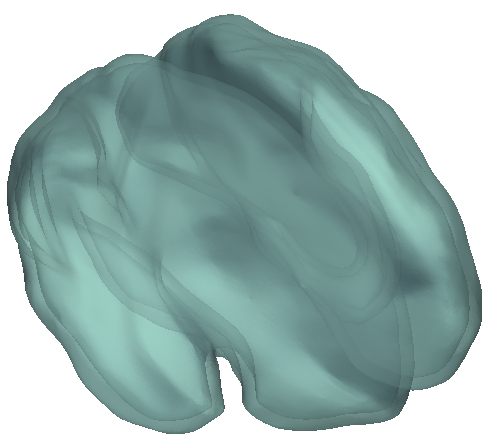
\includegraphics[width=250pt]{template_rendered.png}};
\draw [connection] ([xshift=-50] grb0-west) -- node {\midarrow} (grb0-west);

%%%%%%%%%%%%%%%%%%%%%%%%%%%%%%%%%%%%%%%%%%%%%%%%%%%%%%%%%%%%%%%%%%%%%%%%%%%%%%%%%%%%%%%%
%% Output meshes and images
%%%%%%%%%%%%%%%%%%%%%%%%%%%%%%%%%%%%%%%%%%%%%%%%%%%%%%%%%%%%%%%%%%%%%%%%%%%%%%%%%%%%%%%%
\node[inner sep=0pt] (img-in) at ([xshift=-200, yshift=-100] c1-west)
    {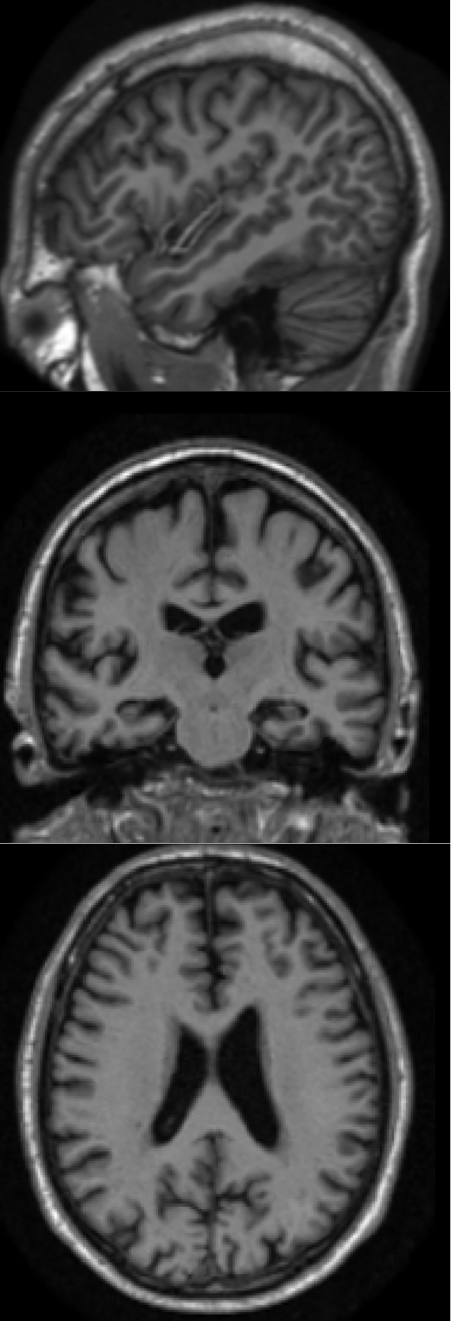
\includegraphics[width=150pt]{mri_3.png}};
\draw [connection] ([xshift=-100] c1-west) -- node {\midarrow} (c1-west);
\node[inner sep=0pt] (img-out-1) at ([xshift=170, yshift=-100] cf-east)
	{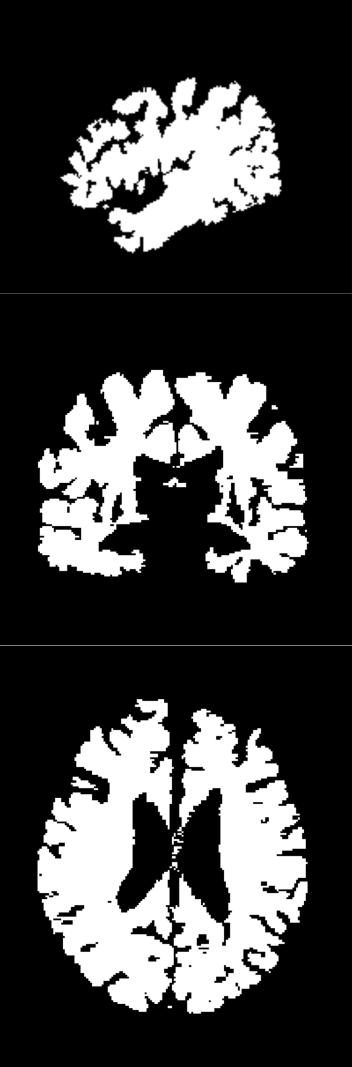
\includegraphics[width=150pt]{seg_binary.png}};
\draw [connection, -Stealth] (cf-east) -- ([xshift=70] cf-east);
\draw [connection, -Stealth] (ds2-east) -- ([xshift=70] ds2-east);
\node[inner sep=0pt] (mout1) at ([yshift=-150, xshift=70] mout-01)
    {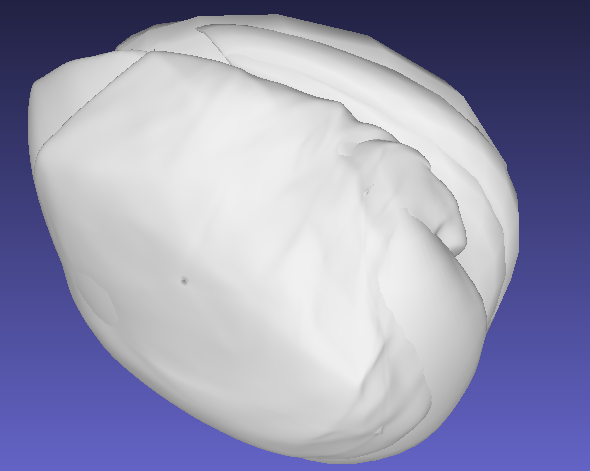
\includegraphics[width=200pt]{step_1.png}};
\node[inner sep=0pt] (mout2) at ([yshift=-150, xshift=70] mout-02)
    {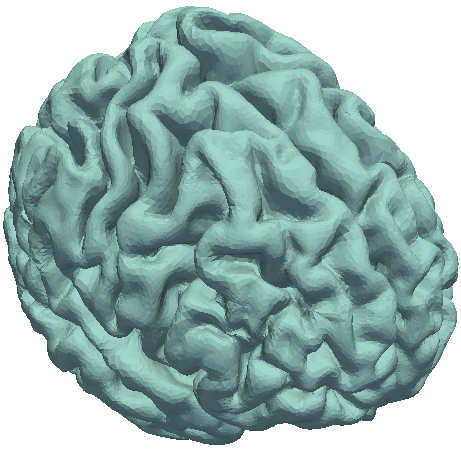
\includegraphics[width=200pt]{step_2.png}};
\node[inner sep=0pt] (mout3) at ([yshift=-150, xshift=70] mout-03)
    {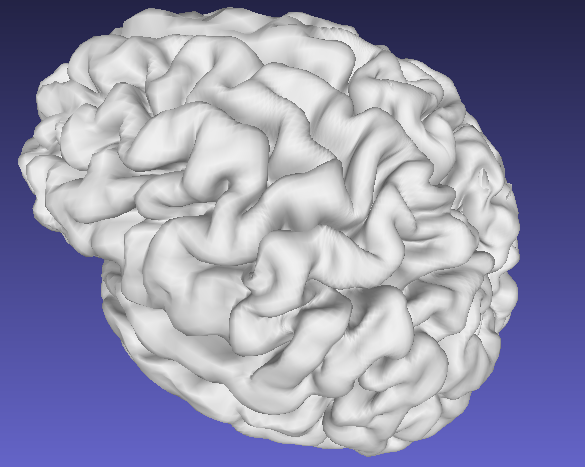
\includegraphics[width=200pt]{step_3.png}};
\node[inner sep=0pt] (mout4) at ([xshift=300, yshift=-20] fv4-east)
    {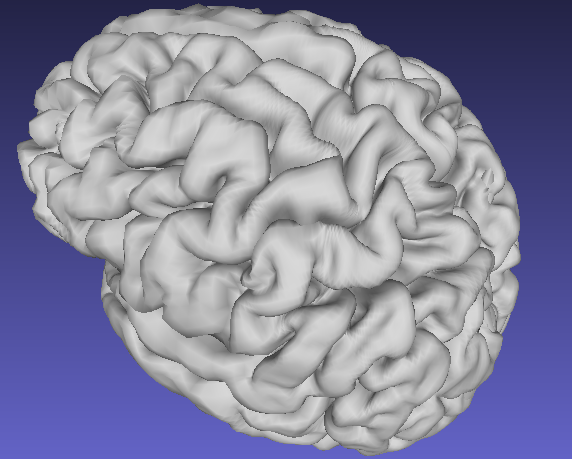
\includegraphics[width=250pt]{step_4.png}};

%%%%%%%%%%%%%%%%%%%%%%%%%%%%%%%%%%%%%%%%%%%%%%%%%%%%%%%%%%%%%%%%%%%%%%%%%%%%%%%%%%%%%%%%
%% Draw legend
%%%%%%%%%%%%%%%%%%%%%%%%%%%%%%%%%%%%%%%%%%%%%%%%%%%%%%%%%%%%%%%%%%%%%%%%%%%%%%%%%%%%%%%%
\tikzset{rectnode/.style = {rectangle, rounded corners=0pt, minimum width = 30pt, minimum height = 30pt}}
\coordinate (legend-northwest) at ([yshift=-170pt,xshift=220pt] template.south);
\matrix[matrix of nodes, nodes={opacity=0.9, draw=none},
	column 2/.style={anchor=west}, draw=black, densely dashed, thick, rounded corners,
        row sep=5pt,column sep=10pt, rectangle] at (legend-northwest) {
		\node[rectnode,fill=ConvColor]{}; &
		\node[fill=none] {\huge Conv 3x3x3, stride 1}; &
		\node[rectnode,fill=ConvReluColor]{}; &
		\node[fill=none] {\huge BatchNorm3d + ReLU}; \\
		\node[rectnode,fill=PoolColor]{}; &
		\node[fill=none] {\huge Conv 2x2x2, stride 2}; &
		\node[rectnode,fill=ConvKOneColor]{}; &
		\node[fill=none] {\huge Conv 1x1x1, stride 1}; \\
		\node[rectnode,fill=UpsampleColor]{}; &
		\node[fill=none] {\huge Upsample trilinear}; &
		\node[rectnode,fill=UnpoolColor]{}; &
		\node[fill=none] {\huge ConvTranspose 2x2x2, stride 2}; \\
		\node[ellipse, minimum size =30pt, fill=GraphConvColor]{}; &
		\node[fill=none] {\huge Graph conv}; &
		\node[ellipse, minimum size =30pt,fill=GraphReluColor]{}; &
		\node[fill=none] {\huge BatchNorm1d + ReLU}; \\
		% Empty row to be filled later
		\node[ellipse, minimum size =30pt, fill=none, name=e-leg1] {}; &
		\node[ellipse, minimum size =30pt, fill=none, name=e-leg2] {}; &
		\node[fill=none, name=e-leg3] {}; &
		\node[fill=none, name=e-leg4] {}; \\
	};
% Multicolumn
\node[ellipse, minimum size = 30pt, fill=FeatureColor1, draw=black, solid] (f1-leg) at (e-leg1.center){};
\node[ellipse, minimum size = 30pt, fill=FeatureColor9] (f9-leg) at (e-leg2.center){};
\node[fill=none, anchor=west] at ([xshift=-165pt] e-leg3.center) {\huge Trilinear interpolation at vertices};
\draw[loosely dotted, line width=5pt, line cap=round, dash pattern=on.5off7] (f1-leg.center) -- (f9-leg.center);
%%%%%%%%%%%%%%%%%%%%%%%%%%%%%%%%%%%%%%%%%%%%%%%%%%%%%%%%%%%%%%%%%%%%%%%%%%%%%%%%%%%%%%%%
\end{tikzpicture}
\end{document}
